\section{Expressões Algébricas}

\subsection{Expressões Algébricas}

A Matemática é uma linguagem e como tal, expressa alguma coisa. Ao calcular a área de um retângulo com \textit{3 cm} de comprimento e \textit{4 cm} de largura, escrevemos $3 \cdot 4$ (três vezes quatro) e estamos expressando a soma de $4 + 4 + 4$.  Tanto $3 \cdot 4$ como $4 + 4 + 4$ são expressões numéricas, cujo significado particular é o número de $cm^2$ do retângulo.

Para escrever de modo geral a área de qualquer quadrado de lado $x$, usamos $x^2$. Esta expressão com \textit{letras} e \textit{números}, chamamos de \textit{expressão algébrica}.

\vspace{5mm}

\settowidth\widest{\textbf{(a)}}
\stepcounter{exemplo}
\begin{description}[leftmargin=\dimexpr\widest+\labelsep\relax,labelindent=0pt,
    labelwidth=\widest]
\item[\textbf{Exemplo~\thesubsection.\theexemplo~-}]

\noindent O lado do quadrado pode ser expresso pela letra  x  e isso significa que o lado é variável, ou seja, pode assumir diferentes valores positivos.

\begin{figure}[h]
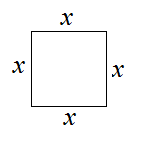
\includegraphics{capitulos/expressoes_algebricas/media/image2.png}
\centering
\end{figure}

\noindent Se \textit{$x = 2$ cm} o quadrado tem todos os lados iguais a \textit{2 cm} e é aproximadamente do tamanho de um ladrilho de revestimento de paredes.

\noindent Se \textit{$x = 2,2$ m}, o quadrado tem todos os lados iguais a $2,2$ \textit{m} e é aproximadamente do tamanho de banheiro.

\noindent Se \textit{$x = 1$ hm} (\textit{100m}), o quadrado tem todos os lados iguais a \textit{1 hm} e é aproximadamente do tamanho de uma quadra de cidade.

\noindent Devemos observar que o lado do quadrado expresso por $x$ é variável, ou seja, pode assumir diferentes valores.

\noindent Para cada valor de $x$ proposto acima, o perímetro (\textit{P}) de todos os quadrados, pode ser escrito com uma equação algébrica:

\begin{center}
\textit{P = 4x.}
\end{center}

\noindent Dizemos que $4x$ é a expressão algébrica do perímetro de qualquer quadrado de lado $x$. Nesse caso, o número $4$ é uma constante (coeficiente, parte numérica) e $x$ é a variável (parte literal) \qedsymbol

\noindent As expressões algébricas recebem nomes específicos em função do número de termos:

\setlength{\parskip}{.5em}
\noindent 1 termo = \textbf{monômios}. Exemplos: $7x^3$; $3m^2n^4$\par
\setlength{\parskip}{0em}
\noindent 2 termos = \textbf{binômios}. Exemplos:  $x+1$; $7x^3 -4x$; $4y - 3$; $x^2 - 1$\par
\noindent 3 termos = \textbf{trinômios}. Exemplos: $x^4 - x^3 + 3$; $x^2$- $2x$ + 3\par
\noindent Mais do que 3 termos = \textbf{polinômios}. Exemplo: $2x^4$ - $3x^3$ + $3x^2$ + 2.

\end{description}

\setlength{\parskip}{.5em}

\textbf{\textit{Definição}}: dois monômios são semelhantes se as partes literais forem idênticas.

\newpage

\stepcounter{exemplo}
\textbf{Exemplo~\thesubsection.\theexemplo~-}
\settowidth\widest{\textbf{(a)}}
\begin{description}[leftmargin=\dimexpr\widest+\labelsep\relax,labelindent=0pt,
    labelwidth=\widest]
\item
\begin{enumerate}[label=(\textbf{\alph*)}]
    \item Os monômios $7x^3$ e $3x^3$ são semelhantes, pois as partes literais são idênticas;
    
    \item Os monômios  $2ab^2$ e $2a^3b$ não são semelhantes, pois as partes literais são diferentes \qedsymbol
\end{enumerate}

\end{description}

\noindent\textbf{EXERCÍCIOS \thesubsection}

\settowidth\widest{\textbf{(a)}}
\begin{description}[leftmargin=\dimexpr\widest+\labelsep\relax,labelindent=0pt,
    labelwidth=\widest]

\stepcounter{exercicio}
\label{e:3.1.1}
\item[\thesubsection.\theexercicio]
Use variáveis para expressar o perímetro e a área de:
\begin{enumerate}[label=(\textbf{\alph*)}]
\item Quadrados
\item Retângulos em que um lado é o dobro do outro
\item Retângulos em que a diferença dos lados é \textit{2 cm}
\item Retângulos em que um lado é \textit{5 cm} maior do outro
\end{enumerate}

\hyperref[r:3.1.1]{Ver Resposta}

\stepcounter{exercicio}
\item[\thesubsection.\theexercicio]
Determine a expressão algébrica do perímetro do retângulo
\begin{figure}[h]
  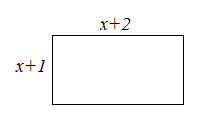
\includegraphics{capitulos/expressoes_algebricas/media/image3.png}
  \centering
\end{figure}

\stepcounter{exercicio}
\item[\thesubsection.\theexercicio]
Determine a expressão algébrica do perímetro da figura:
\begin{figure}[h]
  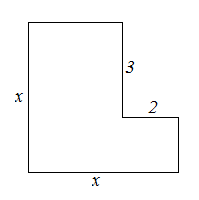
\includegraphics{capitulos/expressoes_algebricas/media/image4.png}
  \centering
\end{figure}

\stepcounter{exercicio}
\item[\thesubsection.\theexercicio]\label{ex:3.1.3}
Determine o perímetro da figura do \hyperref[ex:3.1.3]{\textbf Ex 3.1.3} para $x = 4$.

\stepcounter{exercicio}
\item[\thesubsection.\theexercicio]
O valor de $x$ poderia ser $1$ na figura do \hyperref[ex:3.1.3]{\textbf Ex 3.1.3} ?

\newpage
\stepcounter{exercicio}
\item[\thesubsection.\theexercicio]
Calcule o valor numérico das expressões com os respectivos valores das variáveis:

\begin{multicols}{2}\large
a) $7x^3 + x^2 - 3x + 1$ para $x = -2$\\
b) $ - x^4 + 5x - \frac{1}{3}$ para $x = - 1$\\
c) $\frac{x+1}{x^2-2}$ para $x = 2$\\
d) $\frac{x+1}{x^2-x+1}$ para $x=\frac{1}{2}$
\end{multicols}\normalsize

\end{description}

\subsection{Operações com monômios e polinômios}

\begin{center}\fbox{\begin{minipage}{.9\textwidth}\begin{center}

    \textbf{Adição e subtração de monômios e polinômios}
    
    \vspace{5mm}
    
    Só é possível adicionar ou subtrair monômios semelhantes.\\
    
    \vspace{5mm}
    
    Para adicionar ou subtrair monômios, soma-se ou subtrai-se os coeficientes e mantem-se a parte literal.\\
    
    \vspace{5mm}
    
    Para adicionar/subtrair polinômios, soma-se ou subtrai-se os monômios semelhantes.\\
    
\end{center}\end{minipage}}\end{center}

\stepcounter{exemplo}
\textbf{Exemplo~\thesubsection.\theexemplo~-}
\settowidth\widest{\textbf{(a)}}
\begin{description}[leftmargin=\dimexpr\widest+\labelsep\relax,labelindent=0pt,
    labelwidth=\widest]
\item[]

\begin{enumerate}[label=(\alph*)]
    \item $3x^2 + 5x^2 - 2x^2 = (3+5-2)x^2 = 6x^2$
    \item $5y - 7x - 8y + 6x = (5-8)y + (-7+6)x = -3y - x$
    \item $(x^2 + 5x -3) - ( 2x^2 + 2x -8) = -x^2 + 3x + 5$
\end{enumerate}

\end{description}

\begin{center}\fbox{\begin{minipage}{.85\textwidth}\begin{center}

    \textbf{Multiplicação e divisão de monômios}
    
    \vspace{5mm}
    
    Multiplica-se ou divide-se os coeficientes e usa-se a propriedade da multiplicação/divisão de potências de mesma base para multiplicar a parte literal.
    
\end{center}\end{minipage}}\end{center}

\stepcounter{exemplo}
\textbf{Exemplo~\thesubsection.\theexemplo~-}
\settowidth\widest{\textbf{(a)}}
\begin{description}[leftmargin=\dimexpr\widest+\labelsep\relax,labelindent=0pt,
    labelwidth=\widest]
\item[]

\begin{enumerate}[label=(\alph*)]
    \item $(-3x^2 ) \cdot (7x^2) = -21x^4$
    \item $(25x^4 y^2) \div (5x^2 y) = 5x^2y$
    \item $(10x^2) \div (2x) = 5x$
    \item $(12x^3 + 6x^2 - 5x) \div (-2x) = -6x^2 - 3x + \frac{5}{2}$.   

\end{enumerate}
\end{description}

\stepcounter{exemplo}
\textbf{Exemplo~\thesubsection.\theexemplo~-} Multiplique $12 \cdot 15$ \label{ex:3.2.3}

\begin{description}
\item[Solução:]
Vamos escrever $12 = 10 + 2$ e $14 = 10 + 4$. Para multiplicar usamos a propriedade distributiva da multiplicação em relação à adição:

$(10 + 2) \cdot  (10 + 4) = 10 \cdot 10 + 10 \cdot 4 + 2 \cdot 10 + 2 \cdot 4 = 100 + 40 + 20 + 8 = 168$.

Ou, na forma de algoritmo:
\newpage


\hspace{7mm} 1d + 4u

\hspace{7mm} 10 + 2

\hspace{7mm} ---------

\hspace{7mm} 2d    + 8u

\hspace{-1mm} 1c  + 4d

            ---------------

            1c + 6d + 8u        = 168 u $\qedsymbol$


\end{description}

\stepcounter{exemplo}
\noindent\textbf{Exemplo \thesubsection.\theexemplo~-} Multiplique os polinômios: $(x^3 + 6x^2 - 5x) \cdot (x - 2)$

\begin{description}
\item[\textbf{Solução:}]
A multiplicação de dois polinômios segue o mesmo algoritmo da multiplicação de dois números decompostos como soma, como no \hyperref[ex:3.2.3]{\textbf{Ex 3.2.3}}

\hspace{8mm}$x^3 + 6x^2 - 5x$
                
\hspace{23mm}x – 2
		      			 
\hspace{4mm}------------------------
				
\hspace{4mm} $-2x^3 -12x^2  + 10x$
       		       	          
$x^4 +6x^3 -5x^2 $ 
		                
---------------------------
			
$x^4  +  4x^3  -17x^2  + 10x$ $\qedsymbol$
\end{description}


\stepcounter{exemplo}
\textbf{Exemplo \thesubsection.\theexemplo~-} Divida os polinômios: $(x^3 + 6x^2 - 5x) \div (x - 2)$.

\begin{description}
\item[\textbf{Solução:}]
A divisão de polinômios é semelhante ao algoritmo da divisão de dois números inteiros.

\[
\begin{array}{rl}
x^3 + 6x^2 - 5x & \myrule{x-2} \\
\cline{2-2}
-x^3 + 2x^2~~~~~~~~ & x^2  + 8x \\
------\\
+8x^2-5x\\
-8x^2+16x\\
-----\\
+11x
\end{array}
\]
A divisão dos polinômios dá $x^2  + 8x$ e o resto é $+11x$ $\qedsymbol$

\end{description}

\noindent\textbf{EXERCÍCIOS \thesubsection}

\begin{description}

\stepcounter{exercicio}
\item[\thesubsection.\theexercicio] Explique porque podemos cancelar $a$ em $\frac{a \cdot{} b}{a}$ e não podemos em $\frac{a+b}{a}$.

\stepcounter{exercicio}
\item[\thesubsection.\theexercicio] Verifique se as igualdades são verdadeiras (justifique sua resposta):
\begin{multicols}{2}

\begin{enumerate}[label=\alph*)]

\item $a^2  + a^3  = a5$

\item $x^3  \cdot  x^3 = x^6$

\item $y^3 : y^3 = 1$

\item $2m^2 - 3m^2 = -m^2$

\item $x^3 \cdot x^3 = 2x^6$

\item $10y^3 : 2y^2 = 5y$

\end{enumerate}

\end{multicols}

\stepcounter{exercicio}
\item[\thesubsection.\theexercicio] Resolva as operações com as expressões algébricas:

\begin{multicols}{2}

\begin{enumerate}[label=\alph*)]
    \item $3x^2 + \frac{1}{3}x^2 - 2x^2$
    
    \item $ab^2 - \frac{1}{2}ab^2 + \frac{1}{4}ab^2$
    
    \item $y^3 - \frac{3}{4}y^3 + 2y^3$
    
    \item $x(xy+2x+3y)$
    
    \item $(x-3)(x^2-\frac{1}{3}x+3$
    
    \item $a^2b \cdot ab^3 \cdot a^3b$
    
    \item $(y^2-\frac{1}{5} \cdot (5y-2)$
    
    \item $7a^3b^2x^2 : 14a^2bx$
    
    \item $(2x^3+5x^2+2x) : (x+\frac{1}{2}$
    
    \item $\frac{1}{2}m^3n^2 : \frac{1}{4}m^2n+mn$
\end{enumerate}

\end{multicols}

\stepcounter{exercicio}
\item[\thesubsection.\theexercicio] Dados os polinômios $A = 2x+1$; $B = x-3$ e $C = 2x^2+5x+2$, resolva:

\begin{multicols}{4}

\begin{enumerate}[label=\alph*)]
    \item $A+B$
    
    \item $B+C-A$
    
    \item $A \cdot B$
    
    \item $A \cdot C$
    
    \item $C - x \cdot A$
    
    \item $C:A$
    
    \item $C:B$
    
    \item $A \cdot B-C$
\end{enumerate}

\end{multicols}

\stepcounter{exercicio}
\item[\thesubsection.\theexercicio] Um lado de um retângulo é expresso por $x +3$ e outro por $2x$:

\begin{enumerate}[label=\alph*)]
\item Determine a expressão algébrica do perímetro.

\item Determine a expressão algébrica da área.

\item Para que valor de $x$ o perímetro é $18cm$?

\item Se a área é $56cm^2$, qual é o valor de $x$?

\item Qual é o valor de $x$ para que os lados sejam iguais?
\end{enumerate}

\stepcounter{exercicio}
\item[\thesubsection.\theexercicio] A área de um retângulo é expressa por $x^2+2x-3$ e um dos lados por $x-1$. Determine a expressão algébrica do outro lado.

\stepcounter{exercicio}
\item[\thesubsection.\theexercicio] O lado de um cubo é expresso por $x+1$. Determine a expressão algébrica:

\begin{enumerate}[label=\alph*)]
    \item Do volume
    \item Da área de uma face
    \item Da área superficial
\end{enumerate}

\stepcounter{exercicio}
\item[\thesubsection.\theexercicio] Com base na figura, determine as expressões algébricas do perímetro e da área.

\begin{figure}[H]
~~~~~~~
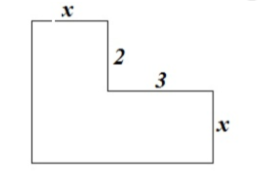
\includegraphics[scale=.8]{capitulos/expressoes_algebricas/media/image5.png}
\end{figure}

\stepcounter{exercicio}
\label{ex:3.2.9} \item[\thesubsection.\theexercicio] O lado de um quadrado é expresso por $x+3$:

\begin{enumerate}[label=\alph*)]
\item Determine a expressão algébrica da área.

\item Calcule a área para $x = 1$.

\item $x$ pode ser zero?

\item Qual o valor de $x$ para que a área seja nula.
\end{enumerate}

\stepcounter{exercicio}
\item[\thesubsection.\theexercicio] Calcule os valores da área do quadrado do \hyperref[ex:3.2.9]{\textbf{Ex 3.2.9}} para $x = {-3,-2,-1,0,1,2,3}$

\end{description}

\subsection{Produtos Notáveis}

Produtos notáveis são produtos especiais de polinômios. São chamados “notáveis” porque aparecem seguidamente em problemas de Matemática.

~~



\textbf{Quadrado da soma de dois termos}: $(a+b)^2 = a^2 + 2ab + b^2$

~~

\textbf{Quadrado da diferença de dois termos}: $(a - b)^2 = a^2 - 2ab + b^2$

~~

\textbf{Produto da soma pela diferença}: $(a + b) \cdot (a - b) = a^2 - b^2$

~~

\textbf{Cubo da soma de dois termos}: $(a + b)^3 = a^3 + 3a^2b + 3ab^2 + b^3$

~~

\textbf{Cubo da diferença de dois termos}: $(a - b)^3 = a^3 - 3a^2b + 3ab^2 - b^3$

~~

\noindent\textbf{EXERCÍCIOS \thesubsection}

\stepcounter{exercicio}
\begin{enumerate}[label=\alph*)]
\begin{multicols}{3}
    \item $(x+5)^2$
    
    \item $(2x-3)^2$
    
    \item $(x+\frac{1}{2})^2$
    
    \item $(3-x)^2$
    
    \item $(\frac{1}{2}x+2)^2$
    
    \item $(x+1)^3$
    
    \item $(2x-5)^3$
    
    \item $(x-3)(x+3)$
    
    \item $(m+3n)(m+3n)$
    
    \item $(x+\frac{1}{2})(x-\frac{1}{2})$
    
    \item $(x+1)(x+2)$
    
    \item $(x-1)(x+3)$
    
    \item $(2a-b)(2a+b)$
    
    \item $(a+b+1)^2$
    
    \item $(x+\frac{1}{4})(x+2)$
\end{multicols}
\end{enumerate}

\subsection{Fatoração}

\begin{center}\fbox{\begin{minipage}{.85\textwidth}\begin{center}

    \textit{\textbf{Fatores} são os termos de uma multiplicação e \textbf{fatorar} é transformar um número ou expressão algébrica em um produto de fatores.}
    
\end{center}\end{minipage}}\end{center}


\begin{description}
\item [Exemplos:] ~
\begin{enumerate}[label=\alph*)]
\item O número 12 fatorado é $3 \cdot 4$ , onde 3 e 4 são fatores.

\item Podemos decompor números em fatores primos, por exemplo: $24 = 2 \cdot2 \cdot 2 \cdot 3$. Os números 2 e 3, nesse caso são fatores, onde o fator 2 aparece três vezes.

\item Na expressão $3x^2a^3$, 3, $x^2$  e $a^3$ são fatores.
\end{enumerate}
\end{description}

\begin{description}
\item [Fatoração com Fator Comum:]~

Algumas expressões algébricas têm \textit{fatores comuns} (fatores que estão presentes em mais de uma expressão algébrica) que se pode colocar em evidência (colocar em separado, na forma de fatores). Vejamos os exemplos:
\begin{enumerate}[label=\alph*)]
\begin{multicols}{2}
\item $3x + 6y = \colorbox{gray}{3}x + 2 \cdot \colorbox{gray}{3}y = 3 \cdot (x+2y)$.

Observemos que o 3 é fator comum aos dois monômios.
\end{multicols}

\begin{multicols}{2}
\item $4ab^3 - 2a^3b + 10ab^4 = 2ab \cdot (2b^2 - a^2 + 5b^3)$.

Observemos  que o 2ab é fator comum aos três monômios
\end{multicols}

\begin{multicols}{2}
\item $2an + 2bn - am - bm$.

\textbf{(Fatoração por agrupamento)}
\end{multicols}

Nos dois primeiros termos o fator comum é $2n$ e nos dois últimos o fator comum é $-m$.

~~

$2an + 2bn - am - bm = 2n(a+b) - m(a+b)$

~~

A expressão resultante tem mais um fator comum: $(a+b)$. Então:

~~

$2an + 2bn - am - bm = (a+b)(2n-m)$. 
\end{enumerate}
\end{description}

\begin{description}
\item [Fatoração do Trinômio Quadrado Perfeito (TQP):]~

Um trinômio é \textit{quadrado perfeito (TQP)} se foi originado pelo quadrado da soma ou subtração de dois termos.

\begin{multicols}{2}
$a^2 + 2ab + b^2 = (a + b)^2$

(\textit{Quadrado da soma de dois termos})
\end{multicols}

\begin{multicols}{2}
$a^2 - 2ab + b^2 = (a - b)^2$

(\textit{Quadrado da diferença de dois termos})
\end{multicols}

Observemos que o trinômio foi \textit{transformado (fatorado)} em um produto onde os fatores são $(a \pm b)$. Chamando $a$ de \textit{“primeiro termo do binômio”} e $b$ de \textit{“segundo termo do binômio”}, dizemos que o trinômio $a^2 + 2ab + b^2$ é o quadrado do primeiro, mais duas vezes o primeiro vezes o segundo mais o quadrado do segundo.

\end{description}

\begin{description}
\item [Fatoração da Diferença de dois quadrados:]~

\begin{multicols}{2}
$a^2 - b^2 = (a+b) \cdot (a - b)$

(\textit{Produto da soma pela diferença de dois termos})
\end{multicols}
\end{description}

\stepcounter{exemplo}
\noindent\textbf{Exemplo \thesubsection.\theexemplo~-} Verifique se $x^2 + 2x + 1$ é um TQP.

\begin{description}
\item [Solução:] Se o trinômio dado é um TQP então o primeiro termo do binômio $(a+b)$ deve ser $a = \sqrt{x^2} = x$  ; o segundo termo do binômio $(a+b)$ deve ser $b = \sqrt{1} = 1$.

\textbf{Teste do segundo termo do trinômio:}  $2 \cdot a \cdot b = 2 \cdot x \cdot 1 = 2x$  deve ser igual ao \textit{segundo termo do trinômio}. O que de fato ocorre, neste caso. Assim,

\begin{center} $(x + 1)^2 = x^2 + 2x + 1$. \end{center}

Portanto, o polinômio dado é um TQP \qedsymbol{}

\end{description}

\stepcounter{exemplo}
\noindent\textbf{Exemplo \thesubsection.\theexemplo~-} Verifique se $x^2 + 2x + 4$ é um TQP.

\begin{description}
\item [Solução:] Se o trinômio dado é um TQP então o primeiro termo deve ser $a = \sqrt{x^2} = x$ e o segundo termo $b = \sqrt{4} = 2$.

\textbf{Teste do segundo termo do trinômio:}  $2 \cdot a \cdot b = 2 \cdot x \cdot 2 = 4x$, que é diferente de 2x. Portanto, o trinômio dado não é um TQP \qedsymbol{}

\end{description}

\stepcounter{exemplo}
\noindent\textbf{Exemplo \thesubsection.\theexemplo~-} Complete o trinômio $x^2 - 4x + 1 = 0$, de modo que obtenha-se um TQP.

\begin{description}
\item [Solução:] Para se obter um TQP na identidade dada, o primeiro termo do binômio $(a+b)$ deve ser $a=\sqrt{x^2}=x$. O segundo termo "$b$" pode ser obtido, sabendo que

\begin{multicols}{2}
\item ~~~~~~~~$2 \cdot x \cdot b = -4x$

\item \textit{(duas vezes o primeiro termo, vezes o segundo termo é igual ao segundo termo do trinômio)}
\end{multicols}

Assim, $b = -2$ e o TQP é $(x-2)^2 = x^2 - 4x + 4$.

Para obter o TQP no lado esquerdo da identidade dada, basta adicionar (+3) em ambos os lados:

~~

$x^2 - 4x +1 +(+3) = 0 +(+3)$

~

$x^2 -4x + 4  = 3$ \qedsymbol{}

\end{description}

\textbf{EXERCÍCIOS \thesubsection}

~~

\stepcounter{exercicio}
\textbf{\thesubsection.\theexercicio ~~~~~~} Fatore as expressões algébricas:

\begin{multicols}{2}
\begin{enumerate}[label=\alph*)]
\item $x^2-x$

\item $a^3b^2-ab+ab^2$

\item $9x^2-12x+4$

\item $9+6x+x^2$

\item $x^2+x+\frac{1}{4}$

\item $x^2-25$

\item $16x^2-\frac{4}{9}$

\item $ax+bx+ay+by$

\item $6+3x+2y+xy$

\item $x^3+1$
\end{enumerate}
\end{multicols}


\stepcounter{exercicio}
\textbf{\thesubsection.\theexercicio ~~~~~~} Verifique se os trinômios são quadrados perfeitos:

\begin{multicols}{2}
\begin{enumerate}[label=\alph*)]
\item $x^2+4x+16$

\item $x^2+6x+9$

\item $4y^2-12y+9$

\item $9x^2-6x+3$
\end{enumerate}
\end{multicols}

\stepcounter{exercicio}
\textbf{\thesubsection.\theexercicio ~~~~~~} Adicione constantes nas equações de modo a obter trinômios quadrados perfeitos no lado esquerdo da igualdade:

\begin{multicols}{2}
\begin{enumerate}[label=\alph*)]
\item $x^2 +6x + 10 = 0$

\item $4x^2 +4x + 3 = 0 $

\item $9x^2 - 12x + 5  = 0$

\item $x^2 + 10x + 12  = 0$
\end{enumerate}
\end{multicols}

\subsection{Expressões algébricas fracionárias}

Expressões algébricas fracionárias são expressões com variáveis no denominador.

~~

\noindent\textbf{Exemplos:}
\begin{multicols}{3}
\begin{enumerate}[label=\arabic*)]{\large
\item $\frac{a+b}{b}$

\item $\frac{x^2+3x+5}{x-1}$

\item $\frac{ab^2-5a+b}{a+b}$

}\end{enumerate}
\end{multicols}

\subsubsection{Menor Múltiplo Comum (MMC) com expressões algébricas:}

Para encontrar o MMC de números são conhecidos dois métodos:

Encontre o MMC(6,8):

\begin{description}
    \item [a) Usando conjuntos de múltiplos:]~
        
    Os múltiplos de 6 são : M(6)={6,12,18,\colorbox{gray}{24},30,36,42,\colorbox{gray}{48},54,60,66,\colorbox{gray}{72},78,...}

    Os múltiplos de 8 são : M(8)={8,16,\colorbox{gray}{24},32,40,\colorbox{gray}{48},56,64,\colorbox{gray}{72},80,...}

    Examinando os conjuntos de múltiplos de 6 e 8, observa-se que existem vários múltiplos comuns, mas o menor deles é 24. Então, MMC(6,8) = 24.
\end{description}

\begin{description}
    \item [b) Usando decomposição em fatores primos:]~
    
    1º) decompor os números em fatores primos;

    2º) o MMC é o produto de todos os fatores, porém aqueles que se repetirem, escolhe-se apenas os de potência maior. 
    
    \begin{multicols}{3}
    $6 = 2 \cdot 3$
    
    e
    
    $8 = 2^3$
    \end{multicols}
    
    Os fatores são 2, 3 e $2^3$ . Como o fator 2 se repetiu, escolhemos apenas $2^3$. 
    
    Então, MMC(6,8) =  $2^3 \cdot 3  = 24$.
 
	O MMC de expressões algébricas é calculado pelo método da decomposição.
\end{description}

\begin{description}
\stepcounter{exemplo}
\item [Exemplo \thesubsection.\theexemplo] Determine o MMC das expressões algébricas:

a) $ab^2 e a^3b$.

Os fatores são: $a$; $a^3$; $b$ e $b^2$. Então, o MMC($ab^2, a^3b$) = $a^3b^2$

b) $x^2+2x+1$ e $2(x+1)$:

Fatorando a primeira expressão, temos: $x^2+2x+1$ = $(x + 1)^2$. 
Os fatores são: $(x + 1)^2$ ; 2 e $(x+1)$. Então o MMC das expressões dadas é $2(x + 1)^2$ \qedsymbol{}

\end{description}

\subsubsection{Operações com frações algébricas}

As operações com frações algébricas seguem as mesmas regras das operações com frações numéricas e polinômios.

\begin{description}
\stepcounter{exemplo}
\item [Exemplo \thesubsection.\theexemplo] Resolva as operações com as frações algébricas:

{\large a) $\frac{a}{b}+\frac{2a}{b^2}$ =}

O MMC($b,b^2$) = $b^2$. Aplicando o algoritmo da adição de frações, temos:

\begin{center}{\large
$\frac{a}{b}+\frac{2a}{b^2}=\frac{ab+2a}{b^2}=\frac{a(b+2)}{b^2}$
}\end{center}

{\large b) $\frac{x}{x+2} \cdot \frac{x+1}{x^2-1}$ =}

Ao invés de multiplicas diretamente, podemos fazer simplificações reescrevendo o denominador da segunda fração como: $(x^2 - 1)$ = $(x+1)(x-1)$. Assim,

\begin{center}{\large
$\frac{x}{x+2} \cdot \frac{x+1}{x^2-1} = \frac{x}{x+2} \cdot \frac{x+1}{(x+1)(x-1)}$ =
}\end{center}

Cancelando os fatores iguais (propriedade do cancelamento), temos:

\begin{center}{\large
$\frac{x}{x+2} \cdot \frac{x+1}{x^2-1} = \frac{x}{x+2} \cdot \frac{1}{x-1} = \frac{x}{(x+2)(x-1)}$ ~~~~
}\qedsymbol{}\end{center}
\end{description}

\begin{description}
\item [EXERCÍCIOS \thesubsection]~~

\begin{enumerate}[label=\textbf{\thesubsection.\arabic*}~~~~]
    \item Simplifique as frações algébricas usando a propriedade do cancelamento:
    
    \begin{multicols}{3}{\large
        \begin{enumerate} [label=\alph*)]
            \item $\frac{21x^4}{15x}$
            
            \item $\frac{x^2}{x^2-x}$
            
            \item $\frac{a^2-a}{a^2-2a+1}$
            
            \item $\frac{y+2}{4y^2-16}$
            
            \item $\frac{x^3+4x^2-21x}{x^2-9}$
            
            \item $\frac{a^3+3a^2-5a-15}{a^2+3a}$
        \end{enumerate}
    }\end{multicols}
    
    \item Resolva as adições e subtrações com frações algébricas:
    
    \begin{multicols}{3}{\large
        \begin{enumerate} [label=\alph*)]
            \item $\frac{1}{3x} + \frac{x+1}{x^2}$
            
            \item $\frac{2}{x} + \frac{1}{x+1} - \frac{x}{x-1}$
            
            \item $\frac{1}{y^2-1} - \frac{1}{y+1}$
            
            \item $\frac{2}{a} + \frac{a}{a^2+1}$
            
            \item $\frac{x}{x+3} + \frac{1}{x^2+6x+9}$
            
            \item $\frac{x}{x^2-25} - \frac{x-1}{2x-10}$
        \end{enumerate}
    }\end{multicols}
    
    \item Multiplique as frações algébricas usando a propriedade do cancelamento:
    
    \begin{multicols}{3}{\large
        \begin{enumerate} [label=\alph*)]
            \item $\frac{4}{x-1} \cdot \frac{x^2-1}{16}$
            
            \item $\frac{x+4}{1-x^2} \cdot \frac{1-x}{x^2-16}$
            
            \item $\frac{1}{x} \cdot \frac{x^2-6x+9}{x+1} \cdot \frac{x^2+x}{x-3}$
            
            \item $\frac{4x^2-2}{x^2} \cdot \frac{6x^2-6}{4x^4-4x^2+1}$
            
            \item $\frac{x^3-1}{2x^2} \cdot \frac{4x}{x^2+x+1}$
            
            \item $\frac{y+3}{7} \cdot \frac{21}{2y+6}$
        \end{enumerate}
    }\end{multicols}
    
    \item Resolva as operações com frações algébricas:
    
    \begin{multicols}{2}{\large
        \begin{enumerate} [label=\alph*)]
            \item {\Large $\frac{\frac{1}{x}}{\frac{x+1}{x^3}}$}
            
            \item $\frac{x}{3x+1} + \frac{x+1}{9x^2-1}$
            
            \item $\frac{a}{a-1} : \frac{a^3}{a^3-a}$
            
            \item $\frac{1}{2y+5} - \frac{y}{4y^2+20y+25}$
            
            \item $\frac{1}{x} \cdot \frac{x^3}{x-2} + \frac{1}{x^2-4}$
            
            \item $\frac{x}{x-3} - \frac{1}{x^2-6x+9} : \frac{6x^2-36x+54}{2x-6}$
        \end{enumerate}
    }\end{multicols}
    
\end{enumerate}
\end{description}

~~

\setcounter{tempi}{0}
\begin{description}
    \item [{\large RESPOSTAS DOS EXERCÍCIOS PROPOSTOS}] ~~
    \begin{enumerate}[label=\textbf{\thesection.\thetempi.\thetempii}]
        \stepcounter{tempi}
        \setcounter{tempii}{0}
        
        \stepcounter{tempii}
        \label{r:3.1.1}
        \item \begin{multicols}{2}
            \begin{enumerate}[label=\alph*)]
                \item $P = 4x;$ $A = x^2$
            
                \item $P = 6x;$ $A = 2x^2$
            
                \item $P = 4x-4;$ $A = x^2-2x$
                
                \item $P = 4x+10;$ $A = x^2+5x$
            \end{enumerate}
        \end{multicols}
        \hyperref[e:3.1.1]{Retornar ao Enunciado}        
        \stepcounter{tempii}
        \item $P = 4x+6$
        
        \stepcounter{tempii}
        \item $P=4x$
        
        \stepcounter{tempii}
        \item $P = 16 cm$
        
        \stepcounter{tempii}
        \item Não. Se $x = 1 cm$, a figura não seria fechada.
        
        \stepcounter{tempii}
        \item \begin{multicols}{4}
            \begin{enumerate}[label=\alph*)]
                \item 45
            
                \item $\frac{-19}{3}$
            
                \item $\frac{3}{2}$
                
                \item 2
            \end{enumerate}
        \end{multicols}
        
        \stepcounter{tempi}
        \setcounter{tempii}{0}
        ~~
        
        \stepcounter{tempii}
        \item Só podemos cancelar quando o mesmo número ou variável está sujeito a operações inversas. Neste caso, a multiplicação por $a$ pode ser cancelada com a divisão por $a$.
        
        \stepcounter{tempii}
        \item \begin{enumerate}[label=\alph*)]
            \item Falsa. A soma dos expoentes, quando as bases são iguais, só é feita se a operação entre as potências for a multiplicação.
            
            \item Verdadeira. Na multiplicação de potências de mesma base conserva-se a base e soma-se os expoentes.
            
            \item Verdadeira. Na divisão de potências de mesma base, conserva-se a base e subtrai-se os expoentes.
            
            \item Verdadeira.
            
            \item Falsa. Multiplica-se os coeficientes ao invés de somá-los.
            
            \item Verdadeira.
        \end{enumerate}
        
        \stepcounter{tempii}
        \item \begin{multicols}{3}
            \begin{enumerate}[label=\alph*)]
                \item $\frac{4}{3}x^2$
                
                \item $\frac{3}{4}ab^2$
                
                \item $\frac{9}{4}y^3$
                
                \item $x^2y+2x^2+3xy$
                
                \item $x^3-\frac{10}{3}x^2+4x-9$
                
                \item $a^6b^5$
                
                \item $5y^3-2y^2-y+\frac{2}{5}$
                
                \item $\frac{1}{2}abx$
                
                \item $2x^2+4x$
                
                \item $3mn$
            \end{enumerate}
        \end{multicols}
        
        \stepcounter{tempii}
        \item \begin{multicols}{3}
            \begin{enumerate}[label=\alph*)]
                \item $3x-2$
                
                \item $2x^2+4x-2$
                
                \item $2x^2-5x-3$
                
                \item $4x^3 + 12x^2 + 9x+2$
                
                \item $4x+2$
                
                \item $x+2$
                
                \item $2x+11;$ $R=35$
                
                \item $-10x-5$
            \end{enumerate}
        \end{multicols}
        
        \stepcounter{tempii}
        \item \begin{multicols}{5}
            \begin{enumerate}[label=\alph*)]
                \item $6x+6$
                
                \item $2x^2+6x$
                
                \item $2cm$
                
                \item $4cm$
                
                \item $3$
            \end{enumerate}
        \end{multicols}
        
        \stepcounter{tempii}
        \item $x+3$
        
        \stepcounter{tempii}
        \item \begin{multicols}{3}
            \begin{enumerate}[label=\alph*)]
                \item $x^3+3x^2+3x+1$
                
                \item $x^2+2x+1$
                
                \item $6x^2+12x+6$
            \end{enumerate}
        \end{multicols}
        
        \stepcounter{tempii}
        \item $P=4x+10;$ $A=x^2+5x$
        
        \stepcounter{tempii}
        \item \begin{multicols}{4}
            \begin{enumerate}[label=\alph*)]
                \item $x^2+6x+9$
                
                \item $16$
                
                \item Sim
                
                \item $-3$
            \end{enumerate}
        \end{multicols}
        
        \stepcounter{tempii}
        \item Respectivamente $0;1;4;9;16;25;36$
        
        \stepcounter{tempi}
        \setcounter{tempii}{0}
        ~~
        
        \stepcounter{tempii}
        \item \begin{multicols}{2}
            \begin{enumerate}[label=\alph*)]
                \item $x^2+10x+25$
                
                \item $4x^2-12x+9$
                
                \item $x^2+x+14$
                
                \item $x^2-6x+9$
                
                \item $\frac{1}{4}x^2+2x+4$
                
                \item $x^3+3x^2+3x+1$
                
                \item $8x^3-60x^2+150x+125$
                
                \item $x^2-9$
                
                \item $m^2+6mn+9n^2$
                
                \item $x^2-14$
                
                \item $x^2+3x+2$
                
                \item $x^2+2x-3$
                
                \item $4a^2-b^2$
                
                \item $a^2+b^2+2ab+2a+2b+1$
                
                \item $x^2+\frac{9}{4}x+\frac{1}{2}$
            \end{enumerate}
        \end{multicols}
        
        \stepcounter{tempi}
        \setcounter{tempii}{0}
        ~~
        
        \stepcounter{tempii}
        \item \begin{multicols}{3}
            \begin{enumerate}[label=\alph*)]
                \item $x(x-1)$
                
                \item $ab(a^2b-1+b)$
                
                \item $(3x-2)^2$
                
                \item $(x+3)^2$
                
                \item $(x+\frac{1}{2})^2$
                
                \item $(x+5)(x-5)$
                
                \item $(4x+\frac{2}{3})(4x-\frac{2}{3})$
                
                \item $(x+y)(a+b)$
                
                \item $(3+y)(2+x)$
                
                \item $(x^2+1)(x-1)$
            \end{enumerate}
        \end{multicols}
        
        \stepcounter{tempii}
        \item \begin{multicols}{2}
            \begin{enumerate}[label=\alph*)]
                \item Não é um TQP.
                
                \item É um TQP: $(x+3)^2$
                
                \item É um TQP: $(2y-3)^2$
                
                \item Não é um TQP.
            \end{enumerate}
        \end{multicols}
        
        \stepcounter{tempii}
        \item \begin{multicols}{4}
            \begin{enumerate}[label=\alph*)]
                \item $-1$
                
                \item $-2$
                
                \item $-1$
                
                \item $13$
            \end{enumerate}
        \end{multicols}
        
        \stepcounter{tempi}
        \setcounter{tempii}{0}
        ~~
        
        \stepcounter{tempii}
        \item \begin{multicols}{3}
            \begin{enumerate}[label=\alph*)]
                \item $\frac{21}{15}x^3$
                
                \item $\frac{x}{x -1}$
                
                \item $\frac{a}{a-1}$
                
                \item $\frac{1}{4y-8}$
                
                \item $\frac{x(x+7)}{x+3}$
                
                \item $\frac{a^2-5}{a}$
            \end{enumerate}
        \end{multicols}
        
        \stepcounter{tempii}
        \item \begin{multicols}{3}
            \begin{enumerate}[label=\alph*)]
                \item $\frac{4x+3}{3x^2}$
                
                \item $\frac{-x^3+2x^2-x-2}{x(x+1)(x-1)}$
                
                \item $\frac{1-(y-1)}{(y+1)(y-1)}$
                
                \item $\frac{3a^2+2}{a(a^2+1)}$
                
                \item $\frac{x^2+3x+1}{(x+3)^2}$
                
                \item $\frac{-x^2-2x+5}{2(x^2-25)}$
            \end{enumerate}
        \end{multicols}
        
        \stepcounter{tempii}
        \item \begin{multicols}{3}
            \begin{enumerate}[label=\alph*)]
                \item $\frac{x+1}{4}$
                
                \item $\frac{1}{x^2-3x-4}$
                
                \item $x-3$
                
                \item $\frac{6(x^2-1)}{x^2}$
                
                \item $\frac{2(x-1)}{x}$
                
                \item $\frac{3}{2}$
            \end{enumerate}
        \end{multicols}
        
        \stepcounter{tempii}
        \item \begin{multicols}{3}
            \begin{enumerate}[label=\alph*)]
                \item $\frac{x^2}{x+1}$
                
                \item $\frac{3x^2+1}{9x^2-1}$
                
                \item $\frac{a+1}{a}$
                
                \item $\frac{y+5}{(2y+5)^2}$
                
                \item $\frac{x^3+2x^2+1}{x}$
                
                \item 1
            \end{enumerate}
        \end{multicols}
        
    \end{enumerate}
\end{description}